\documentclass[a4paper,11pt]{report}
%\documentclass[dvips]{seminar}
\usepackage{pslatex}
\usepackage{graphicx}
\usepackage{longtable}
\usepackage[usenames]{color}
\pagestyle{plain}
%\textwidth=26cm
%\textheight=19.0cm

\begin{document}
%\setlength{\oddsidemargin}{-.01cm}
%\setlength{\topmargin}{-2.cm}

\begin{center}
{\huge \bf \color{red} BigDFT User Manual}\\
\vskip 2em
{\Large \color{red} http://inac.cea.fr/L\_Sim/BigDFT}
\end{center}

\vskip 5em

\large
\begin{itemize}
\item Stefan.Goedecker@unibas.ch, {\normalsize http://www.unibas.ch/comphys/comphys}
\item Luigi.Genovese@esrf.fr
\item Damien.Caliste@cea.fr
\item Alessandro.Mirone@esrf.fr
\item Thierry.Deutsch@cea.fr
\end{itemize}

\normalsize
\tableofcontents

\chapter{Installing BigDFT}

The compilation and installation of BigDFT relie on the GNU standard building chain: 'configure', 'make', 'make install'. BigDFT can be used as an independent program (as described in this manual), or as a library, to be embeded in other softwares, like inside ABINIT.

\section{Building the executables}

\subsection{Configure}
BigDFT build system is based on standard GNU autotools. The end
user does not need to have the autotools package installed on his
computer, the \texttt{configure} script provided in BigDFT package
will do the job to create the \texttt{Makefile} and set the
options, like the optimisation level, the associated libraries to link
with, and so on.

After the package has been untarred, the sources should be configured, depending on the system we
want to run on. Thanks to the autotools, it is possible to generate several builds from the same
source tree. It is advised to create a compilation directory, either inside or outside the source tree. Lets call this directory \texttt{compile-gFortran} for instance. One starts the configure from there \texttt{'source tree path'/configure}.

One can tune the compilation environment using the following options:
\begin{itemize}
  \item \texttt{FC}: Specify the compiler (including MPI aware wrappers).
  \item \texttt{FCFLAGS}: Specify the flags, like the
optimisation flags, to pass to the compiler (default are \texttt{-g
-O2} for GNU compilers).
  \item Linear algebra options:
  \begin{itemize}
    \item \texttt{--with-ext-linalg}: Give the name of the libraries replacing BLAS and LAPACK (default = none specified). Use the -l before the name(s).
    \item \texttt{--with-ext-linalg-path}: Give the path of the other linear algebra libraries (default = \texttt{-L/usr/lib}). Use the -L before the path(es).
  \end{itemize}
  \item Accelarators:
  \begin{itemize}
    \item \texttt{enable-cuda-gpu}: Compile CUDA support for GPU computing.
    \item \texttt{--with-cuda-path}: Give the path to the NVIDIA CUDA tools (default is \texttt{/usr/local/cuda}).
    \item \texttt{--with-nvcc-flags}: Specify the flags for the NVIDIA CUDA Compiler.
    \item \texttt{--enable-opencl}: Compile OpenCL support for GPU computing (compatible with \texttt{--enable-cuda-gpu}).
    \item \texttt{--with-ocl-path}: Give the path to the OpenCL installation directory (default is \texttt{/usr}).
  \end{itemize}
  \item Optional libraries:
  \begin{itemize}
    \item \texttt{--with-etsf-io}: Use ETSF file format (binary based on NetCDF) for densities, potentials and wavefunction files.
    \item \texttt{--with-archives}: Use compression (tar.bz2) for position files during geometry optimisation.
  \end{itemize}
  \item \texttt{--prefix=DIR}: Specify your installation directory (\texttt{/usr/local} is default).
\end{itemize}

An example of compilation using the MKL from Intel instead of basic BLAS and LAPACK installation:\\
\texttt{../configure --with-ext-linalg="-lmkl\_ia32 -lmkl\_lapack"\\
   --with-ext-linalg-path="-L/opt/intel/mkl72/lib/32"\\
   --prefix=/home/caliste/usr FC=ifort}

\smallskip

An other example, compiling CUDA parts:\\
\texttt{../../sources/bigdft-1.3.0-dev/configure\\
  FC=mpif90 FCFLAGS="-O2  -assume 2underscores"\\
  CC=icc CXX=icc CXXFLAGS="-O2  -I/applications/cuda-2.2/include/"\\
  CFLAGS="-O2  -I/applications/cuda-2.2/include/"\\
  --with-ext-linalg="-L/applications/intel/mkl/lib/em64t\\
                     -lmkl\_scalapack\_lp64 -lmkl\_blacs\_intelmpi20\_lp64\\
                     -lmkl\_intel\_lp64 -lmkl\_lapack -lmkl\_sequential -lmkl\_core"\\
  --enable-cuda-gpu --with-cuda-path=/applications/cuda-2.2}

The other options available can be browsed via the \texttt{--help} option.
Some of them are listed here (and they can be of course combined with each other, when it does make sense):
\begin{itemize}
  \item \texttt{--disable-mpi}: Force not to use MPI during build. By default the configure will try to detect if the compiler has some native MPI capabilities. If not MPI will be automatically disabled.
\item \texttt{--enable-debug}: Creates a slower version of the executable in which any of the array allocated is filled by \texttt{NaN} after its boundaries. Useful to detect runtime errors during developments
\item \texttt{--with-memory-limit=<mem>}: Creates a version of the executable which abort the run if one of the processes allocates more memory than \texttt{<mem>} (in Gb). This version is not necessarily slower that traditional copilation.
\end{itemize}


\subsection{Make}
Make the package and create the 'bigdft' executable, issuing \texttt{make}. The GNU option \texttt{-j$n$} is working with whatever value of $n$ (tested up to 16).

\subsection{Install}
To install the package, issue \texttt{make install}. It will copy all files to the specified prefix (see configure).

\subsection{Clean}
Clean the source tree of the 'make' action by \texttt{make clean}.

\section{Building a library}
To avoid to create the binary executable,
use \texttt{--disable--build-binary} option.

The main subroutine of the BigDFT package is the \texttt{call\_bigdft} routine. For a given set of input coordinates 
and input parameters it returns the total energy and the forces acting on the nuclei. The \texttt{BigDFT.f90} main program 
calls the \texttt{call\_bigdft} routine and can also do a geometry optimization by calling the \texttt{geopt} routine (which in turn calls 
again \texttt{call\_bigdft}). For other standard applications other main programs exist.
At present main programs to do a vibrational analysis, saddle point search and global optimization have been developed.
Users are encouraged to write their own main programs for specific applications. 
The BigDFT API will be the object of a forthcoming chapter.

\chapter{File formats and conventions in BigDFT}
\section{The basis set}
\subsection{One dimensional functions}
The maximally symmetric Daubechies family of degree 16 is used to represent 
the Kohn-Sham orbitals. The two fundamental functions of this family, 
the scaling function $\phi$ and the wavelet $\psi$ are shown in Fig. \ref{sym_16} 
for the one-dimensional case.
To form a basis set these functions have to be centered on the nodes of a regular grid.
\begin{figure}[ht]
\begin{center}
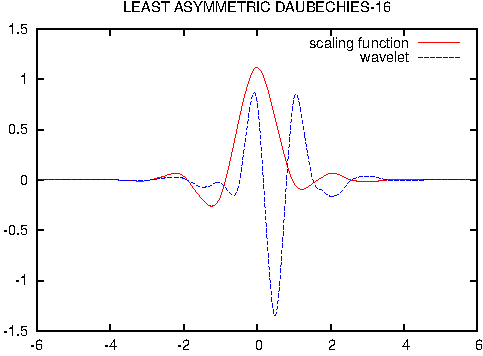
\includegraphics[width=\textwidth]{sym_16.pdf}
\end{center}
\label{sym_16}
\caption{Daubechies Scaling Function and Wavelet of order 16}
\end{figure}
\subsection{Wavelet basis sets in three dimensions}
A 3-dim wavelet basis is made by products of 1-dim functions.
 {\color{red} 1  scaling function} and {\color{blue} 7 wavelets} 
can be centered on the nodes (i,j,k) of a regular 3-dim Cartesian grid.
They all are products of 1-dim scaling functions and wavelets:
\begin{eqnarray*}
 {\color{red} \phi_{i,j,k}(x,y,z) }  & = & \phi(x-i) \phi(y-j) \phi(z-k)   \\
 {\color{blue} \psi^1_{i,j,k}(x,y,z) } & = & \phi(x-i) \phi(y-j) \psi(z-k)  \\
 {\color{blue} \psi^2_{i,j,k}(x,y,z) } & = & \phi(x-i) \psi(y-j) \phi(z-k)  \\
 {\color{blue} \psi^3_{i,j,k}(x,y,z) } & = & \phi(x-i) \psi(y-j) \psi(z-k)  \\
 {\color{blue} \psi^4_{i,j,k}(x,y,z) } & = & \psi(x-i) \phi(y-j) \phi(z-k)  \\
 {\color{blue} \psi^5_{i,j,k}(x,y,z) } & = & \psi(x-i) \phi(y-j) \psi(z-k)  \\
 {\color{blue} \psi^6_{i,j,k}(x,y,z) } & = & \psi(x-i) \psi(y-j) \phi(z-k)  \\
 {\color{blue} \psi^7_{i,j,k}(x,y,z) } & = & \psi(x-i) \psi(y-j) \psi(z-k)  \\
\end{eqnarray*}
If a grid point carries the 7 {\color{blue} wavelets} in addition to the {\color{red} scaling function}, it belongs 
to the high resolution region. In the low resolution region a grid point carries only 
a single {\color{red} scaling function}. In the high resolution region, the resolution is doubled 
in each direction with respect to the low resolution region. The grid spacing is specified by the parameters
{\bf hgridx}, {\bf hgridy}, {\bf hgridz}. The low resolution region is constructed in the following way. Around each 
atom one draws a sphere whose radii are the 'size of the atom' times the adimensional parameter {\bf crmult}. All the grid 
points being contained in the union of all these spheres form the low resolution region. The high resolution is 
constructed in a similar way. One draws spheres whose radii are the 'size of the bonding region' times the 
parameter {\bf frmult} around each atom.  All the grid points being contained in the union of all these spheres 
form the high resolution region. Default values for the 'size of the atom' and  the 'size of the bonding region' 
are contained in the package. The user can however choose different values and these values can be specified by 
adding an additional line at the end of the pseudopotential parameter files which contain first the alternative 
values of {\bf crmult} and then {\bf frmult}.

\subsection{Visualizing the simulation grid with V\_Sim package}
The grid can be visualized by calling the \texttt{memguess} program 
with the option {\bf y}. Then the output file 'grid.xyz' contains the atomic positions and in addition 
the grid points which denoted by 'g' if the are in the coarse region and by 'G' if they are in the fine region. 
Whereas the total number of basis functions is nearly independent of the orientation of the molecule, the size of some 
work arrays depends on the orientation. When the \texttt{memguess} routine is called with the option {\bf o}, it will rotate 
a molecule that will be calculated with free boundary conditions in such a way that the simulation cell size and 
hence the size of the work arrays are as small as 
possible. The rotated output is written in the file posout\_000.xyz.

\begin{figure}[ht]             % produce figure
\begin{center}
\begin{tabular}{cc}
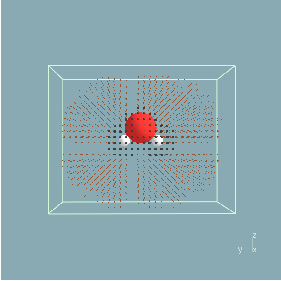
\includegraphics[width=0.4\textwidth]{grid100.pdf} &
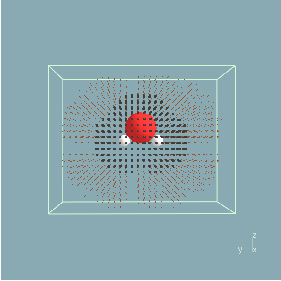
\includegraphics[width=0.4\textwidth]{grid200.pdf} \\
frmult=8 crmult=4 hgrid=.5 & frmult=12 crmult=4 hgrid=.5 \\
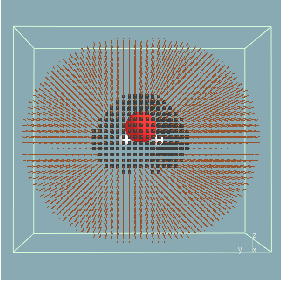
\includegraphics[width=0.4\textwidth]{grid300.pdf} &
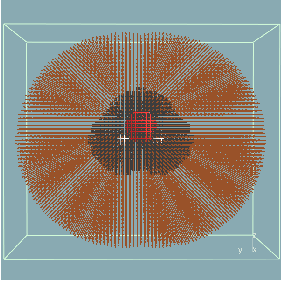
\includegraphics[width=0.4\textwidth]{grid400.pdf} \\
frmult=12 crmult=6 hgrid=.5 & frmult=12 crmult=6 hgrid=.3
\end{tabular}
\end{center}
\label{grids}
\caption{Illustration of the grid and its parameters}
\end{figure}

\section{Format of Input/Output files for atomic coordinates} 
BigDFT supports atomic files which are of two types.
The first one is a particular generalisation of the traditional \texttt{.xyz} format and can be obtained from this via simple modifications.
The second one (\texttt{.ascii}) is peculiar of BigDFT and V\_Sim. Both formats work with the two codes.
\subsection{The \texttt{.xyz} format}
By default the atomic input coordinates are in the file \texttt{posinp.xyz}.
If the same operation (\textit{e.g.} geometry optimization) 
has to be done for several structures one can also give a list of input files whose names (without the .xyz extension) 
have to be contained in a file '\texttt{list\_posinp}'. The first line in the '\texttt{list\_posinp}' file has to be the number of input 
files and each consecutive line contains then one filename.

All the input and output files for atomic coordinates are in the \texttt{.xyz} format, \textit{i.e.} they can be visualized with any 
standard visualization package and in particular with V\_Sim. The first line contains the number of atoms 
and then the units, which are specified by 'atomic', 'atomicd0' or 'Bohr' if atomic units are used or by 
'angstroem' or 'angstroemd0' if the angstr\"om unit is used. 'd0' formats (\texttt{1pe24.17} in Fortran) guarantee that not a single bit is 
lost during write and read of the numbers.

The second line contains the boundary conditions specified by the keywords 'free' for free boundary 
conditions, 'periodic' for periodic boundary conditions or 'surface' for surface boundary conditions
where the x and z direction have periodic boundary conditions and the y direction free boundary conditions. 
The keywords 'periodic and 'surface' have to be followed by 3 real numbers giving the length of the 
orthorhombic periodic cell. In the case of surface boundary condition the second of these numbers is ignored.

The following lines contain the name of the chemical element followed by the $3$~Cartesian coordinates. 
Chemical elements are identified by their pseudopotential. If a element is for instance denoted by 
'Si' the element will be described by the file 'psppar.Si' which has to be present in the working directory.
of the BigDFT.run. A silicon atom could however also be denoted by 'Si\_lda' if there is file 'psppar.Si\_lda.
BigDFT supports the GTH and HGH pseudopotentials in the format which can be downloaded from the ABINIT website
(www.abinit.org). The $3$~Cartesian coordinates can be followed by optional additional information.

In the case of spin-polarized calculation the polarization in the region around the atom can 
be given by an integer. In addition the charge in the region around the atom can be specified.
Finally it can be specified if the atom is fully or partially fixed during a geometry optimization.
'\texttt{f}' stands for completely frozen, '\texttt{fxz}' if the atom can only move along the y axis and '\texttt{fy}' if the atom 
can only move in the XY plane. Below are some examples:

This hydrogen atom is frozen during the geometry optimization
\begin{verbatim}
  H  1.2  3.4  5.6   f
\end{verbatim}

This hydrogen atom has a spin up polarization
\begin{verbatim}
  H  1.2  3.4  5.6   1
\end{verbatim}

This chlorine atom has an additional electron and no spin polarization
\begin{verbatim}
  Cl  1.2  3.4  5.6   0  -1
\end{verbatim}

Same as above, but also frozen
\begin{verbatim}
  Cl  1.2  3.4  5.6   0  -1   f
\end{verbatim}

\subsection{The \texttt{.ascii} format}
BigDFT can also use another text file format for input (and thus output) atomic positions. Here is its structure:

\begin{itemize}
  \item 1st line is arbitrary
  \item 2nd line must contain dxx dyx dyy values
  \item 3rd line must contain dzx dzy dzz values other lines may contain: 
  \begin{itemize}
    \item keywords, with the syntax [\#!]keyword: followed by a list of keywords, separated by commas or blank spaces.
    \item comments beginning with '\#' or '!'
    \item x y z name [label] for atomic position and optional labels
  \end{itemize}
\end{itemize}

dxx dyx dyy dzx dzy dzz values define the box that contains the atoms. The format allows non-orthogonal boxes, but BigDFT supports only orthorombic super-cells, so dyx, dzx and dzy must be zeros. When the keyword angdeg is used, the six values contains the three lengths of basis vectors in dxx dyx and dyy, and the three angles (bc, ac, ab) in dzx dzy and dzz.

After the three first mandatory lines, all subsequent lines can be comment lines (ignored), \textit{i.e.} empty, containing only blanks, or beginning with ! or with \#. A non comment line must contain 'x y z name', giving the 3 coordinates and the name of the atom. The coordinates of the atoms are given in the orthonormal basis not in the box basis. In case the keyword reduced has been specified, the three coordinates x, y and z are given in the box basis.

The keywords can be positionned anywhere after the first three lines. The following list summurises all available keywords:
\begin{itemize}
  \item \texttt{reduced}: All atomic coordinates are given in reduced coordinates with respect to the box definition.
  \item \texttt{angdeg}: The box definition contains three distances and three angles instead of the classical six projection values.
  \item \texttt{bohr} or \texttt{bohrd0}: The units for the distance are Bohr.
  \item \texttt{angstroem} or \texttt{angstroemd0}: The units for the distance are Angströms.
  \item \texttt{atomic} or \texttt{atomicd0}: The units for the distance are Bohr.
  \item \texttt{periodic}, \texttt{surface} or \texttt{freeBC}: The periodicity of the system is either 3D, 2D (free direction is y) or 0D.
\end{itemize}

Additional informations can be provided after the atom names, like for the \texttt{.xyz} format.

%\pagebreak
\section{The input file '\texttt{input.dft}'}
This file contains all the parameters required for a single wavefunction calculations:
\begin{itemize}
\item {\bf hgridx}, {\bf hgridy}, {\bf hgridz}: The grid spacing of the Cartesian grid, in Bohr. As 
       described above the nodes of this grid serve as the centers for the scaling function/ wavelet basis. 
       Values are in most cases between $.3$ and $.6$.

\item {\bf crmult}, {\bf frmult}: Coarse Region Multiplier and Fine Region Multiplier which serve to determine the radius
      for the low/high resolution sphere around the atom. 
      Values are typically of the order of 5 for {\bf crmult} and of the order of 10 for  {\bf frmult}.
\item {\bf ixc}: integer specifying which exchange correlation functional will be used. The Abinit conventions are 
      used and detailed information can be found on the Abinit Web page 
      (www.abinit.org/documentation/helpfiles/for-v5.8/in\-put\_variables/varbas.html\#ixc). 
      Here is only a short summary of some wide\-ly used functionals:\\
      \begin{tabular}{rl}
      {$1$}       & Pade LDA from Abinit XC library;\\
      {$11$}      & PBE from Abinit XC library;\\
      {$-020$}    & Pade LDA from libXC;\\
      {$-101130$} & PBE from libXC;\\
      {$-116133$} & PBEsol from libXC; \\ 
      {$-406$}    & PBE0 Hybrid functional (local part from libXC).
      \end{tabular}
      A positive integer refers to a functional from ABINIT library and a negative one from libXC
      library. In this case, you concatenate the codes for the exchange part and for the correlation part
      (see the table in appendix~\ref{appendix-libXC}).
%\item {\bf ncharge}, {\bf elecfield}: Total charge of the system and constant electric field along the y direction in units of Ha/Bohr. 
\item {\bf ncharge}, {\bf elecfield}: Total charge of the system and uniform electric field $E_x,E_y,E_z$ in units of Ha/Bohr. 
      A positive {\bf ncharge} means that electrons are taken away. 
      The electric field can not have components in periodic directions, e.g. $E_x=E_z=0$ in case surface BC is used.
\item {\bf nspin}, {\bf mpol}: 
      nspin=1, closed shell system without spin polarization;\hfill\\
      nspin=2: spin polarized system; 
      nspin=4: non-collinear magnetic system.
\item {\bf gnrm\_cv} convergence criterion for the wavefunction optimization (norm of the gradient).
      Reasonable values are in most cases between 1.d-4 and 1.d-5.
\item {\bf itermax}, {\bf nrepmax}: Maximum number of gradient evaluations for a single cycle in a wavefunction optimization 
      and maximum number of cycles. At the end of each cycle a subspace diagonalization is done which helps 
in cases where one has near degeneracy between the HOMO and LUMO orbitals. $50$~and $2$~are usually sufficient.
\item {\bf ncong}, {\bf idsx}: ncong gives the number of iterations in the solution of the preconditioning equation.
      For free boundary conditions $5$ is a good value whereas for other  boundary condition a value from 0 to 2 is in general sufficient. 
      Large values of {\bf ncong} lead to a smaller number of iterations in 
      the wavefunction optimization and better forces, but each iteration is more costly. 
      So an optimal compromise value has to be found.
      {\bf idsx} gives the history length of the DIIS convergence acceleration in the wavefunction optimization.
      6 is usually a good value for fast convergence.\\
      In case of convergence problems it can be advantageous 
      to switch off DIIS by setting {\bf idsx} = 0. The memory requirements grow considerably with large values of 
      {\bf idsx}. If memory is the limiting factor one has to choose {\bf idsx} smaller than the value which gives 
      the fastest convergence. The '\texttt{memguess}' tool can be used to predict the memory requirements for different choices 
      of  {\bf idsx}.
\item {\bf dispersion}:  A non-zero values activates an  empirical add-on treatment of dispersion effects.
      The values~1, 2~and 3~specify different switching on functions using the convention of 
      Q. Hill and C.-K. Skylaris.  Proc. R. Soc. A 465  (2009) 669
\item {\bf InputPsiId }, {\bf  output\_wf},  {\bf output\_density }: 
      {\bf InputPsiId } specifies how the input guess wavefunction is generated:
      \begin{itemize}
      \item {\bf InputPsiId } = -2: Random numbers are used as input guess. This is of course a poor input guess which will 
            need many iterations of the wavefunction optimization and might even lead to divergences.
      \item {\bf InputPsiId } = -1: The input wavefunction is imported from the CP2K code which
            uses Gaussian functions. 
            The basis set should be contained in a file named \texttt{gaubasis.dat} 
            whereas the coefficients should appear in the \texttt{gaucoeff.dat} file. 
            Both files are the output files of CP2K code. See the H2O-CP2K test for an example.
      \item {\bf InputPsiId } = 0: A subspace diagonalization in a minimal atomic basis set is used.
            This input guess should be used in general if one starts a new calculation. 
      \item {\bf InputPsiId } = 1: The previously calculated wavefunctions (for instance from the previous 
            geometry optimization step) are used as input guess. Setting {\bf InputPsiId } to 
            this value does only make sense from within a main program where \texttt{call\_cluster} was 
            called previously. The old wavefunction is passed to the new call via the data structure 'restart'
      \item {\bf InputPsiId } = 2: The input wavefunction is read from the 'wavefunction.*' files which contain all the 
            scaling function and wavelet coefficients. In case some parameters such as {\bf hgridx} 
            or {\bf crmult} have changed, compared to the previous run, the wavefunctions will be 
            also transformed to the new parameter set. Use also this value to restart from ETSF file format wavefunction-etsf.nc.
      \item {\bf InputPsiId } = 10: The same as 0 but activates the 'Gaussian help': 
            after convergence the wavefunctions are projected onto the localised basis set used for
            the input guess, and Mulliken Charge Population Analysis (MCPA) is performed on this
            basis. The user has the possibility to perform MCPA with separate basis set (functionality to be added)
       \item {\bf InputPsiId } = 11: Restart with Gaussian approximation contained in the 'restart' data structure.
       \item {\bf InputPsiId } = 12: The input wavefunction is read from the 'wavefunctions.gau'  file, which contains an 
            approximation in a minimal Gaussian basis set of the previously calculated wavefunctions.
       \item {\bf output\_wf} = 0, Do not write the wavefunctions to disk.
       \item {\bf output\_wf} = 1, The output wavefunctions are written at the end of the wavefunction optimization 
            into plain text files. If {\bf InputPsiId } was greater than 10 the wavefunction will be written 
            in the Gaussian approximation into  a single 'wavefunctions.gau' file otherwise into 
            'wavefunction.*' files. Writing a  'wavefunction.*' file for each orbital can take a considerable 
            amount of time and disk space. 
       \item {\bf output\_wf} = 2, The output wavefunctions are written at the end of the wavefunction optimization 
            into Fortran binary files. This format is not portable between compilers and machines. 
       \item {\bf output\_wf} = 3, The output wavefunctions are written at the end of the wavefunction optimization 
            into ETSF binary files. This format is portable between compilers and machines since based on NetCDF. Parallel IO are taken into account.
       \item {\bf output\_density} = 0, No output density is written.
       \item {\bf output\_density} = 1, Output electronic density is written in the .pot format of V\_Sim into the file 'electronic\_density.pot' (Deprecated, use 11 instead).
       \item {\bf output\_density} = 2, In addition to the electronic density, the potential ('local\_potential.pot') and its components ('ionic\_potential.pot' and 'Hartree\_potential.pot') are also output in plain text '.pot' files (Deprecated, use 12 instead).
       \item {\bf output\_density} = 11, Same as {\bf output\_density} = 1, but files are writtent in ETSF file format (portable binary format based on NetCDF).
       \item {\bf output\_density} = 12, Same as {\bf output\_density} = 2, but files are writtent in ETSF file format (portable binary format based on NetCDF).
       \item {\bf output\_density} = 21, Same as {\bf output\_density} = 1, but files are writtent in '.cube' file format (plain text).
       \item {\bf output\_density} = 22, Same as {\bf output\_density} = 2, but files are writtent in '.cube' file format (plain text).
%  %       \item {\bf output\_denpot} = 0, No output density or potential is written.
%  %       \item {\bf output\_denpot} = 1, Output electronic density and electrostatic potential are written in the .cube format, respectively,  into the files 'electronic\_density.cube' and 'electrostatic\_potential.cube' (Deprecated, use 11 instead).
%  %       \item {\bf output\_denpot} = 2, In addition to the electronic density and the electrostatic potential the components of the potential                ('external\_potential.cube' which has contributions both from ions and electric field, 'Hartree\_potential.cube' and 'XC\_potental.cube') 
%  %         are also output in plain text '.cube' files (Deprecated, use 12 instead).
%  %       \item {\bf output\_denpot} = 11, Same as {\bf output\_denpot} = 1, but files are written in ETSF file format (portable binary format based on NetCDF).
%  %       \item {\bf output\_denpot} = 12, Same as {\bf output\_denpot} = 2, but files are written in ETSF file format (portable binary format based on NetCDF).
%  %%%%       \item {\bf output\_denpot} = 21, Same as {\bf output\_denpot} = 1, but files are written in '.cube' file format (plain text).
%  %%%%       \item {\bf output\_denpot} = 22, Same as {\bf output\_denpot} = 2, but files are written in '.cube' file format (plain text).
      \end{itemize}
\item {\bf rbuf}, {\bf ncongt}:  Far reaching tails of the wavefunctions decaying into the vacuum are  
      added in a perturbative treatment if the variable {\bf rbuf} is set to a strictly positive value. 
      This allows to do a calculation with some moderate 
      value of {\bf crmult} and then to extrapolate to the limit of large  {\bf crmult}. 
      This procedure is not variational and gives too low energies. The true energy is 
      in between the two energies and in general much closer to the extrapolated energy. 
      This procedure can also be used to judge whether the chosen value of  {\bf crmult} is 
      large enough for a certain required precision.
      {\bf rbuf} gives the amount by which the radii for the coarse resolution region 
      are increased in atomic units. {\bf ncongt} gives the number of iterations used 
      in the perturbation calculation. Reasonable values for {\bf ncongt} are around 30.  

\item {\bf norbv},{\bf nvirt}, {\bf  nplot}: Usually unoccupied orbitals are not calculated since they are not needed for 
      the total energy and other physical properties of the electronic ground state. 
      Putting  {\bf norbv} to  a non-zero 
      value will result in the calculation of {\bf norbv} virtual orbitals in a postprocessing 
      routine after the occupied orbitals have been calculated, which uses Davidson iterative treatment . {\bf nplot}  of these 
      orbitals will be written in the 'virtual.*.pot' files and {\bf nplot} (if that many exist) 
      of the highest occupied orbitals will be  written in the 'orbital.*.pot' file
      The Kohn Sham eigenvalues are written in the ordinary output file.  {\bf nvirt} corresponds to the actual number of orbitals the convergence process is taking care of during the Davidson iterations.

\item {\bf verbosity}: Determines the amount of output from little (0)
      to detailed (2). By adding 10 to its value it switch on the
      once-and-for-all strategy for calculating the PSP projectors, which
      is faster but more memory demanding (considered by \texttt{memguess}).
\item \textbf{disable sym}: a logical to set to 'T' to disable the
      usage of symmetry operations in the calculations. By default symmetries
      are used to update the density in periodic boundary condition
      calculations, and surface boundary conditions also.
\end{itemize}

\section{The input file '\texttt{input.geopt}'}
If this file exists, BigDFT will do a geometry optimization and the file contains all the required parameters.

\begin{itemize}
\item {\bf geopt\_approach}: This character string specifies the method used for the geometry optimization.
      \begin{itemize}
      \item  \emph{VSSD}:  Variable Stepsize Steepest Descent method;
      \item  \emph{SDCG}: A combination of Steepest Descent and Conjugate Gradient;
      \item  \emph{LBFGS}: Limited Memory BFGS;
      \item  \emph{BFGS}: Preconditioned steepest descent with energy feedback.
                          A preconditioning matrix is build up according to the  BFGS algorithm.
                          The initial Hessian is a diagonal matrix where the diagonal elements are the 
                          inverse of the step size. This method is usually the most efficient one.
      \item  \emph{PBFGS}: Same as BFGS except that an initial Hessian is obtained from a force field.
                           Force field parameters are only available for systems consisting of H,C,N,O.
                           For such systems the method is the most efficient one in general
      \item  \emph{AB6MD}: The molecular dynamic routines from ABINIT~6.
      \end{itemize}
\item {\bf  ncount\_cluster\_x}: Maximum number of force evaluations to be used for the geometry optimization.
\item {\bf frac\_fluct}, {\bf forcemax}: Convergence criteria for the geometry optimization. 
      The geometry optimization stops either 
      if the norm of the individual forces acting on any atom in the system is smaller than {\bf forcemax} 
      or if the forces get noisy. Noise is present because of the underlying integration grid.
      The parameter {\bf frac\_fluct} specifies how small the forces should become 
      compared to the noise level to stop the geometry optimization. 
      Values in between  1 and 10 is are reasonable for this parameter. 
      A value of 2 means that the geometry optimization will stop when 
      the largest atomic force is comparable to the 2 times the average noise in 
      the forces themselves. For values of  {\bf frac\_fluct} 
      smaller than 1 one can under certain circumstances obtain better relaxed geometries but 
      one risks that the geometry optimization will not converge since the forces are too noisy. 
      In such a case one should 
      closely monitor the progress of the geometry optimization by looking at the 'posout.*' 
      files which are written at each step of the geometry optimization and at the 'geopt.mon' file. 
\item {\bf randdis}: This parameter allows to add random displacements 
      with amplitude \textbf{randdis} to the atomic positions in the 
      input file 'posinp'. This can for instance be useful to break degeneracies (which would lead to 
      convergence problems in the wavefunction optimization) in highly symmetric structures.
\item {\bf betax}: This is the stepsize for the geometry optimization. 
      This stepsize is system dependent and it has therefore to be 
      determined for each system. If the VSSD method is used one can start with a small stepsize of around 1 and 
      VSSD will suggest than a better value for {\bf betax} in the last line of the 'geopt.mon' file. 
      Whether the stepsize is correct can also be seen from the 'geopt.mon' output of the SDCG method. In this 
      case the average stepsize in terms of \textbf{betax} should be around~$4$
      (after a brief initial period where it is around 8).
      In contrast to the SDCG method, the BFGS method is not very sensitive to the correct stepsize but nevertheless 
      one should try to find reasonable values also in this case.
\item \textbf{ionmov}: in case of {\bf geopt\_approach = AB6MD}, the {\bf betax} line should be replaced by this one. It contains an integer value as described in the ABINIT manual. Possible values are:
      \begin{itemize}
      \item 6: simple velocity-Verlet molecular dynamic.
      \item 7: quenched molecular dynamic, when the scalar product force / velocity becomes negative, 
            the velocity is set to zero. The force criterion is tested at each step.
      \item 8: Nose-Hoover thermostat.
      \item 9: Langevin dynamic (adding a friction force and a Gaussian random force on atoms).
      \item 12: Isokinetic ensemble molecular dynamics. The equation of motion of the ions in contact with a thermostat are solved with the algorithm proposed by Zhang [J. Chem. Phys. 106, 6102 (1997)], as worked out by Minary et al [J. Chem. Phys. 188, 2510 (2003)]. The conservation of the kinetic energy is obtained within machine precision, at each step.
      \item 13: Iosthermal/isenthalpic ensemble. The equation of motion of the ions in contact with a thermostat and a barostat are solved with the algorithm proposed by Martyna, Tuckermann Tobias and Klein [Mol. Phys., 1996, p. 1117].
      \end{itemize}
\item \textbf{dtion}: the time step for molecular dynamic, in atomic time units. One atomic time unit is 2.418884e-17 seconds, which is the value of Planck's constant in Hartree*sec. The following lines depend on the choosen value for \textbf{ionmov}.
\item  if \textbf{ionmov = 6}: one line containing the initial temperature in kelvin. If negative, the initial velocities are all zero. If positive, random speeds are chosen to match the given temperature (NOT IMPLEMENTED YET!).
\item  if \textbf{ionmov $>$ 7}: one line containing two temperatures in kelvin. When different, the temperature is linearly change at each geometry step to go from the first value to the second.
\item  if \textbf{ionmov = 8}: one additional line containing the thermostat inertia coefficient for Nose-Hoover dynamic.
\item  if \textbf{ionmov = 9}: two additional lines containing first the friction coefficient and then a value in Bohr corresponding at a distance where the atoms can bounce on (see the ABINIT documentation for further details).
\item  if \textbf{ionmov = 13}: several additional lines containing first the number of thermostats in the chain of thermostats. Then a line with the mass of each thermostat in the chain. And finally a line with two values for the barostat mass, depending on optcell value (NOT IMPLEMENTED YET!).
\end{itemize}


\section{The input file '\texttt{input.kpt}'}
This file is used to specify a set of $k$ points. If this file does not exist, only the $\Gamma$ point will be used. The $k$ point generation relies on the ABINIT implementation. This files contains the following information:
\begin{itemize}
  \item  \textbf{kptopt}: This character string specifies the method used to generate the $k$ point mesh.
       \begin{itemize}
       \item  \emph{auto}: Automatic generation is used, based on the $k$ point density we wish in Fourier space, taking into account the symmetries of the system.
       \item  \emph{MPgrid}: A Monkhorst-Pack grid, using only the special $k$ points, taking into account the symmetries of the system.
       \item  \emph{manual}: A manual set of $k$ points.
       \end{itemize}
       The following lines depend on the choice of \textbf{kptopt}.
  \item  if \textbf{kptopt = 'auto'}: One additional line containing a real space length \textbf{kptrlen}. BigDFT will automatically generate a large set of possible $k$ point grids, and select among this set, the grids that give a length of smallest vector LARGER than \textbf{kptrlen}, and among these grids, the one that, reduces to the smallest number of $k$ points.
  \item  if \textbf{kptopt = 'MPgrid'}: Several additional lines. The first line should contains three integers describing the mesh of Monkhorst-Pack grid in reciprocal space. The second line contains one integer \textbf{nshiftk} that give the number of shift one would like to apply to the MMP grid to obtain the final $k$ point mesh. Then the file contains \textbf{nshiftk} lines with three real numbers each, giving the shift to apply in reciprocal space.
  \item  if \textbf{kptopt = 'manual'}: Several additional lines. The first contains \textbf{nkpt}, an integer giving the number of manually defined $k$ points. Then \textbf{nkpt} lines follow, with four real values each, the three first being the coordinates in reciprocal space (in $[0;0.5]$) and the fourth bing the weight. If the sum of all weights does not equal to one, weight values are renormalised.
\end{itemize}
After the regular $k$ point mesh for the self-consistent loop, one can
define in addition a specific path of $k$ points to be used to compute
a band diagram. This requires also to define Davidson usage in the
'\texttt{input.dft}' file. The band structure is define if the following lines
are present:
\begin{itemize}
  \item \textbf{bands} keyword: a character string containing
\emph{bands}.
  \item the next line contains one integer, \textbf{nseg}, the number
of different segments for the path.
  \item the next line contains \textbf{nseg} integer values, defining
the number different $k$ points to be generated in each segment.
  \item then follow \textbf{nseg + 1} lines containing each three floating
point values with the coordinates of the vertices in reduced
coordinates of the Brillouin zone.
\end{itemize}

\section{The input file '\texttt{input.mix}'}
If this file is present, the SCF loop is run with a diagonalisation scheme instead of the direct minimisation scheme. This file controls how the density or the potential is mixed between each iteration of diagonalisation. It must contain the following lines:
\begin{itemize}
  \item \textbf{iscf}: An integer giving the mixing scheme and the mixing target. It follows the ABINIT convention. For values lower than 10, the potential is mixed, while for values greater than 10, the density is mixed.
  \item \textbf{itrpmax}: Maximum number of diagonalisation iterations.
  \item \textbf{rpnrm\_cv}: The stop criterion on the residue of potential or density.
  \item \textbf{norbsempty Tel}: The number of additional bands and the electronic temperature.
  \item \textbf{alphamix alphadiis}: The multiplying factors for the mixing and for the electronic DIIS.
\end{itemize}

Each diagonalisation step is done with a direct minimisation scheme at a fixed potential. The parameters of this minimisation are the usual ones in the \texttt{input.dft} file. The overall convergency of the diagonalisation is not very sensitive to the good convergency of the direct minisation steps. Thus a itermax value of 5 in \texttt{input.dft} is often advicable.

\section{The input file '\texttt{input.perf}'}
This file is used to specify values in order to optimize the performances of BigDFT. If this file
does not exist, default values are used. On the contrary to other BigDFT input file, this file has optional key / value entries. The keywords are not case sensitive. Keywords can specify options as:
\begin{itemize}
  \item  \textbf{'debug' T/F}: The debug mode is enable mainly for memory profiling.
  \item  \textbf{'fftcache' ncache\_size}: Specify the cache size for FFT in kBytes.
  \item  \textbf{'accel' NO/CUDAGPU/OCLGPU}: Specify the use of CUDA (resp. OCL) versions of various subroutines. For CUDA, a 'GPU.config' file is needed.
  \item  \textbf{'blas' T/F}: Use or not the CUBlas acceleration.
  \item  \textbf{'projrad' real}: Radius of the projector as a function of the maxrad.
  \item  \textbf{'exctxpar' key}: Exact exchange parallelisation scheme.
  \item  \textbf{'ig\_diag' T/F}: Input guess: (T:Direct, F:Iterative) diagonalisation of Hamiltonian.
  \item  \textbf{'ig\_norbp' int}: Input guess: Orbitals per process for iterative diagonalisation.
  \item  \textbf{'ig\_blocks' int int}: Input guess: Block sizes for orthonormalisation.
  \item  \textbf{'ig\_tol' real}: Input guess: Tolerance criterion.
  \item  \textbf{'methortho' key}: Orthogonalisation (0=Cholesky,1=GS/Chol,2=Loewdin).
  \item  \textbf{'rho\_commun' key}: Density communication scheme.
\end{itemize}

\chapter{ Running BigDFT executables}

\section{Estimating the memory usage: \texttt{memguess}}
Before running BigDFT, it is recommended to run the '\texttt{memguess}' program. If it runs correctly all input files are available 
(this routine needs a posinp.xyz and does not accept a list\_posinp file). It then allows to estimate the required memory and to 
find an optimal number of MPI processes for a parallel run. For good load balancing each MPI process should roughly treat the same number of orbitals.

The '\texttt{memguess}' program prints out the number of orbitals and how many orbitals are treated by each MPI process. 
On a parallel machine with a high performance interconnect network one can choose the number of MPI processes {\bf nproc} equal 
to the number of occupied orbitals, \textit{i.e.} each MPI process treats one orbital. On machines with slower networks each MPI process should 
have at least 2 to 4 orbitals.

\texttt{memguess <nproc> [option]}

\begin{itemize}
\item {\bf nproc}: Number of MPI processes;
\item {\bf o}: The molecule will be rotated such that the size of the workarrays is minimal;
\item {\bf y}: Generate a file 'grid.xyz' containing the coarse and the fine grid points;
\item {\bf GPUtest <nrep>}: Case of a CUDAGPU calculation, to test the speed of 3d operators <nrep> is the number of repeats.
\item {\bf upgrade}: Ugrades input files older than 1.2 into actual format;
\item {\bf convert <from.[cube,etsf]> <to.[cube,etsf]>}: Converts file "from" to file "to" using the given formats;
\item {\bf atwf <ng>}: Calculates the atomic wavefunctions of the first atom in the gatom basis and write their expression in the "gatom-wfn.dat" file, <ng> is the number of gaussians used for the gatom calculation.
\end{itemize}

\section{Single point or geometry optimization: \texttt{bigdft}}
The MPI version is executed on most machines with the \texttt{mpirun} command followed by the name of the executable which is 
\texttt{bigdft} in our case.
The treatment of each orbital can be speeded up by using the mixed MPI/OpenMP implementation 
where each MPI processes uses several OpenMP threads to do the calculations for its orbitals faster. 
The OpenMP is simply activated by compiling the program with an OpenMP flag and by specifying the number of OpenMP threats by
export \textbf{OMP\_NUM\_THREADS=4} if 4 threads are for instance desired.

\noindent
The BigDFT program monitors during a run the memory utilization and the time spent in various subroutines. Detailed information 
is written in the files 'malloc.prc' and 'time.prc'. At the end the program checks whether the number of deallocations was equal 
to the number of allocations and whether the total memory went back to zero. If this should not be the case please send a bug report to the developers of BigDFT.

\section{Doing a path minimization: \texttt{NEB}}
A NEB implementation is present in the BigDFT package, thanks to the initial routines provided by Carlos Sbraccia. This implementation is launched with the help of the \texttt{NEB} executable. This program is responsible for initialising the path from the two minima and then to run the path minimisation, using BigDFT to compute the forces. Each replica is launched by an instance of \texttt{bigdft} and not in the same program \texttt{NEB}. This allows to run the NEB algorithm on a super computer with a queue system, each replica going separately in the queue. 
The process of running the different \texttt{bigdft} instances, in different directories and wait for their completions is done by two shell scripts: \texttt{NEB\_driver.sh} and \texttt{NEB\_include.sh}. The first one is very generic and should not be touched by users. It is provided in the \texttt{src/} directory of the package. The second one must be adapted by users to suit to their running machine. One example is provided in the \texttt{tests/NEB/} directory of the package.

The \texttt{NEB} executable can be run from everywhere but the scripts \texttt{NEB\_driver.sh} and \texttt{NEB\_include.sh} must be in the same directory. It takes arguments from the command line, using a redirection from a file is good practice. See the \texttt{tests/NEB} directory of the package:
\begin{center}
  \texttt{./NEB < input}
\end{center}
The file \texttt{input} contains a list of variables relevant to the NEB algorithm. Some of them are explained here:
\begin{itemize}
  \item \texttt{scratch\_dir} is where the \texttt{NEB\_driver.sh} script will create the directories where to run the \texttt{bigdft} instances. It is usually on a local disk.
  \item \texttt{job\_name} a name that will be used to named all generated files and directories.
  \item \texttt{climbing} when set to \texttt{.TRUE.}, the highest replica follow opposite parallel forces in addition to the usual perpendicular ones.
  \item \texttt{optimization} when set to \texttt{.TRUE.}, tries to optimize the geometry of the first and last replicas (if not local minima already).
  \item \texttt{minimization\_scheme} specifies the scheme used to minimze the NEB. The possible values are 'steepest\_descent', 'fletcher-reeves', 'polak-ribiere', \hfill\\ 'quick-min', 'damped-verlet' and 'sim-annealing'.
  \item \texttt{tolerance} is a criterion not to take into account in the list of moving atoms the ones that move less than this value between the first and the last replica.
  \item \texttt{convergence} is the stop criterion on perpendicular forces, in eV/\AA.
  \item \texttt{num\_of\_images} is the number of desired replicas.
  \item \texttt{*\_config} the file describing the first and the last replica (in BigDFT 1.3, the file extension .xyz must be omitted).
\end{itemize}

At each NEB iteration, the driver script is run. It creates the directories for forces calculations if needed, create the input files using the include script, run the jobs, grep the energy and the forces and return. The script file \texttt{NEB\_include.sh} must contain the following shell functions:
\begin{itemize}
  \item \texttt{init\_jobs()}, run once after directory creation. It can be used.
  \item \texttt{finalise\_jobs()}, run once after all jobs have finished.
  \item \texttt{wait\_jobs()}, run each time the script poll all replicas for completion.
  \item \texttt{make\_input()}, run once in each scratch directories to create the file 'posinp.xyz' from the NEB restart file and the initial ones.
  \item \texttt{run\_job()}, run once in each scratch directories to start the force calculations. In the example, it runs the replicas directly on the host machine, but in this shell function, a submission file may be created instead and submitted to the queue system for later run.
  \item \texttt{check\_job()} is used periodically by the driver system to check if a job is finished or not. It must return different values: -1 if the job is still not started (maybe be still in the queue for instance), 0 if the job is running but not finished yet, 1 if it exited with success and 2 if it exited with a failure.
  \item \texttt{grep\_forces()} is run once after job termination to get the energy and the forces. Energy must be in Hartree and forces in Hartree per Bohr.
  \end{itemize}
For NEB purposes, users of BigDFT usually have only to modify the \texttt{run\_job()} functions from the examples to adapt it to their machine.

The output files are:
\begin{itemize}
  \item \texttt{job\_name.NEB.dat}: A three column file containing for each replica a reaction coordinate, the energy in eV and the maximum value of remaining perpendicular forces. This file is updated at each iteration.
  \item \texttt{job\_name.NEB.log}: A file, giving for each NEB iteration the value of the highest replica in eV and the value of the maximum perpendicular forces on all atoms and replicas.
  \item \texttt{job\_name.NEB.restart}: A file with the coordinates of each replicas. This file is generated by the \texttt{NEB} executable at each iteration and used by the driver script to generate the 'posinp' files.
\end{itemize}


\section{Doing frequencies calculations: \texttt{frequencies}}
Using the executable \texttt{frequencies}, it is possible to calculate the vibrational properties of
a system by finite difference. The atomic system is moving for each direction and each atom in a
small step in order to calculate the Hessian matrix by a finite difference scheme.
A checkpoint restart is implemented. The file 'frequencies.res' contains the previous calculations.

\subsection{The '\texttt{input.freq}' file}
There are three parameters:
\begin{itemize}
\item \texttt{freq\_alpha} to determine the step for frequency step (i.e. alpha*hx, alpha*hy, alpha*hz);
\item \texttt{freq\_order} which determines the order of the finite difference scheme:
      \begin{itemize}
      \item $-1$ calculates $\frac{f(x_0)-f(x_0-h)}{h}$;
      \item $1$ calculates $\frac{f(x_0+h)-f(x_0)}{h}$;
      \item $2$ calculates $\frac{f(x_0+h)-f(x_0-h)}{2h}$ (this is the default);
      \item $3$ calculates $\frac{f(x_0+2h)+f(x_0+h)-f(x_0-h)-f(x_0-2h)}{6h}$.
      \end{itemize}
\item \texttt{freq\_method} which determines the method (only 1 at the present stage).
\end{itemize}


\chapter{XANES calculations}

\section{Abstract} 
We have implemented an original procedure for calculating XANES spectra within the BigDFT code. Our approach consists firstly in  projecting the photoelectron wave-function onto the pseudopotential functions basis with the help of a reversed PAW projector\cite{Taillefumier} and, then, propagating this initial state by iterative applications of the Hamiltonian. The Hamiltonian is the one provided by the BigDFT code. The obtained spectra therefore correspond exactly to the electronic structure of the self consistent ground state.The spectra are built by obtaining at each new application of the Hamiltonian a new coefficient of the spectral decomposition in Chebychev polynomials. The method therefore systematically improves the calculated spectra resolution at each step and can be stopped once the required resolution is reached. Moreover, the Chebychev polynomials have a higher nodes' density at the extrema of the spectral range  than in the middle. For practical applications this makes convergence even faster because the broadening due to lifetime is narrow near the edge and large elsewhere. The execution times represent a break-through for this kind of calculations and reflect the exceptional features of the BigDFT code. For a cluster contained in a 25\AA\ side cube, the spectra are obtained within half an hour, running on a single processor.


\section{Introduction}

The interaction between matter and a photon described by a wave vector ${ k}$ and polarisation ${ \epsilon}$,
  is written, discarding elastic Thomson scattering (the $ A^2(r)$ term in the Schr{\"o}dinger equation which becomes dominant off-resonance), discarding also the spin-magnetic field interaction~\cite{blume}, and using CGS units,  as :
\begin{equation}
H_{int} =
 \left( 
   \displaystyle \frac{2 \pi \hbar c^2 }{ \omega V}\right)^{1/2}
   ({  a^\dagger }_{ k,\epsilon} exp(-i {{\bf k} \cdot {\bf r}} ) 
    + a_{k ,\epsilon} exp(i { {\bf k} \cdot {\bf  r}} ))\frac{e}{ m c} {  {\bf p} \cdot  {\bf \epsilon} } \label{fondamentale}
\end{equation}

where ${ r}$ is the electron coordinate, ${ p}$ the kinetic moment, ${  a^\dagger }_{ k,\epsilon}$, $a_{ k ,\epsilon}$ 
are creation annihilation photon operators, $\omega= kc $, and $V$ is the space volume.

The photon absorption is  a first order perturbative process whose probability  per unit of time $w(\omega)$, 
for photon with polarization  $\epsilon$  state, 
is obtained from  $H_{int}$  matrix elements by the Fermi golden rule. For one photon in the $V$ volume:
\begin{equation}
  w(\hbar \omega) = \frac{(2 \pi)^2 e^2 \hbar }{\hbar \omega  V m^2 }  \sum_n  \left|< n |  exp(i { {\bf k} \cdot {\bf  r}} ) { {\bf  p} \cdot  {\bf \epsilon} } | 0 >\right|^2   \delta( \hbar \omega-E_n) 
\end{equation}
where $<n|$ is a complete set of eigenstates of matter, $<0|$  being the initial state, $ E_n$ is the energy difference between $<n|$ and $<0|$  and we have retained only the resonating denominator. 
The absorption cross section is the quantity directly observable in experiment. It is obtained from the above equation dividing by the photon flux  $c/V$:
\begin{equation}
  \sigma(\hbar \omega) = \frac{(2 \pi)^2 e^2 \hbar }{\hbar \omega   m^2 c }  \sum_n  \left|< n |  exp(i { {\bf k} \cdot {\bf  r}} ) { {\bf  p} \cdot  {\bf \epsilon} } | 0 >\right|^2   \delta( \hbar \omega-E_n) 
\end{equation}

The matrix element can be simplified in terms of ${\bf r}$ by using the following identity for  ${\bf p}$:
\begin{eqnarray}
 exp(i {  k \cdot r} ) {  p \cdot  \epsilon }
 & \simeq & ( 1 + i    k \cdot  r + ...  ) \frac{i m}{\hbar} [ H, {  r \cdot  \epsilon }] \\ 
 & = &
  \displaystyle\frac{i m}{\hbar} ([ H, {  r \cdot  \epsilon }] + i [ H, {  k \cdot r}  {  r \cdot  \epsilon }] /2 + ...) \label{expansion} \nonumber
\end{eqnarray} 

Such substitution leads to:

\begin{equation}
  \sigma(\hbar \omega) = (2 \pi)^2  \alpha_0   \hbar \omega    f(\hbar \omega)
\end{equation}

with 

\begin{equation}
  f(\hbar \omega)  =  \sum_n  \left| < n | i > \right|^2   \delta( \hbar \omega-E_n) \nonumber
\end{equation}


where 

\begin{equation}
  |i> = { {\bf  r} \cdot  {\bf \epsilon} }  + i\frac{( { \bf k \cdot r})(  {\bf  r \cdot  \epsilon })}{2} +... | 0 > 
\end{equation}

is the state resulting from the application of the interaction operator on the ground state.

 The $f(\hbar \omega)$ is formally determined by its distribution moments
which can be computed by iterative applications of the Hamiltonian :
\begin{equation}
  \int  f(E) E^n d E = \left| < i | H^n| i > \right|
\end{equation}

To avoid numerical ill-conditioning coming from the numerical linear dependence of  high order powers we proceed as explained in \cite{weiss}.
 The $H$ Hamiltonian is rescaled  and shifted to a new $H'$ whose spectra
is comprised within $]-1,1[$:
$$   < n | H' | n > \in \,\, ]-1,1[ $$
The overlap integrals between the spectra and Chebychev polynomials $T_n(x)$ is calculated by recurrence.
The Chebychev polynomials $T_n(x)$ are:
$$  T_n(x) = cos( n * arccos(x)) $$
and satisfy the recurrence relation:

$$ T_{m+1}(x) = 2 x T_m(x) - T_{m-1} (x)$$

The overlap integral are:
$$\mu_n =  \int  f'(x) T_n(x) = < i |  T_n(H') | i > | $$

and can be obtained by applying the recurrence relation to the left side of $|i>$ state:

$$ T_{m+1}(H')| i > = 2 H' T_m(H')| i > - T_{m-1} (H')| i > $$
and then obtaining the scalar product. The spectra is finally recovered as:

$$  f( b+a x) = \frac{  (\mu_0+ 2 \sum_{n=1}^{\inf} \mu_n T_n(x)) }{a \pi \sqrt{1 - x^2} } $$

where $b$ and $a$ are the shift and the scaling factor respectively, involved in the $ H' \rightarrow H $ transformation.
The spectra can be obtained up to an arbitrary degree of resolution by
applying iteratively the recurrence relation for a sufficient number of times. To avoid oscillation
due to the truncation of the summation, a convolution is applied multiplying the $\mu_n$ 
components by the Jackson kernel~\cite{weiss}. 


\section{Use of the code}

The binary executable for absorption spectra calculation is named \texttt{abscalc}.
 Besides the usual files which  are needed for
a basic BigDFT calculation,  \texttt{abscalc} needs to find, 
 in the current  work directory, at least the file  '{\texttt{input.abscalc}}'. 
This file is specific to absorption calculations and 
its structure will be explained here.
The  usual files needed for a basic BigDFT calculation and by \texttt{abscalc} are, 
we recall it here: '{\texttt{input.dft}}', '{posinp.xyz}', and the pseudopotential files '{psppar.XX}' for
all the elements entering in the structure.

Others files may be needed when one selects the option of importing
the self consistent potential from a previous SCF calculation, as will
be explained later. 

Concerning the '{posinp.xyz}' file we suggest, for a good result,
to set a large box diameter of about $25$\AA\ or more, and periodic
boundary conditions.

The structure of the file '{\texttt{input.abscalc}}' is the following:

\begin{itemize}
\item The input parameter {\it in\%iabscalc\_type} which can be equal to  $1$
or $2$. In the first case the spectra is calculated as a series of
Chebychev polynomials, while in the second case the Lanczos
tridiagonalisation is applied. We suggest the first option
because the Lanczos method requires, in order to keep orthogonality,
 that all the vectors of the tridiagonal base be stored in memory
and this limits the number of steps that one can perform.

\item The  parameter {\it in\%iat\_absorber}, an integer number,
is the position (starting from one) in  the {\it posinp.xyz} file
of the absorber atom.
%({\it WARNING levare gnrm che non serve piu} )

\item  {\it in\%L\_absorber} : this parameter is the angular moment
of the multipole component of the interaction operator that 
one wants to consider. It is $1$ for dipole interaction, $2$ for
quadrupolar ...

\item {\it in\%Gabs\_coeffs(i), i=1,2*in\%L\_absorber +1}.

This are the components of the interaction operator, in Cartesian
coordinates. These correspond to the BigDFT internal representation 
of tensors, which is based on spherical tensor. 
%({\it aggiunger un link o una spiegazione per il caso di L  generico })
For dipolar interaction these will be therefore the three $x,y,z$
components. In this present version the input are real numbers.
Entry for the imaginary parts will have to be added in the future versions 
for magnetic dichroism.

\item   {\it in\%potshortcut } : This parameter determines how the 
local potential is obtained. If it is set to $1$ the potential is
obtained from the superposition of atomic charges.
If it is set to $2$ the potential is read from a previous SCF
calculation. In this case the program searches, in the current work directory,
the file {\it b2B\_xanes.cube}. Such file contains the atomic positions
and the local potential of a previous SCF run and can be created
setting the parameter {\it in\%output\_grid} to $-2$ in
the file {\it \texttt{input.dft}}. The SCF potential is interpolated, using
interpolant wavelets, to get the potential on the target grid.
The SCF grid of the previous run must have less points than the target
grid.
This is easily the case, because in XANES calculations one usually
sets a large diameter for the box. The fact of choosing a large box 
limits the spurious oscillations due to bands effects and to interference with the replica
of the absorber atom in the other Bravais cells. 

\item {\it in\%nsteps } : this is the total number of Hamiltonian
  applications. The larger this number, the better the resolution you get
  in the calculated spectra.

\end{itemize}


\subsection{Note about the absorber pseudopotential}
 In the actual version of the code ($1.4$) for the absorber
pseudopotential one must use a $Z+1$ approximation.
For future versions of the code the development of on-the fly
pseudopotentials, corresponding to the excited electronic structure,
is foreseen.
%{\it verificare che non saranno invece tabulati } 


\section{Description of the output}

In case of  {\it in\%iabscalc\_type} equal to  $1$, the spectra
is written, in the current work directory, with the name :
{\it  cheb\_spectra\_NUM  } where {\it NUM} is the number of 
Chebychev components. The number of components increases
at each Hamiltonian application and ,during the calculation,
 several partial results, with increasing number of components,
 are written.

 % 320 4399475 


\section{The reversed PAW method}

The BigDFT code, in the actual version as well as in the previous
ones, uses a norm-conserving pseudo-potential.
From this pseudo-potential we extract the corresponding
PAW projector.
This is the reverse of the PAW method. In the PAW method 
the projector determines the pseudopotential. In our case
instead, the PAW projector is a function of the pseudo-potential.
The implementation of such function is detailed here.
We need to construct the projector for the absorber atom only
because the core orbitals don't overlap other atoms.
For the absorber atom we proceed by calculating 
the SCF solution in the isolated atom case, once using pseudo-potentials,
and another using the all-electrons potential.
Then, for these potentials, we calculate an almost-complete set 
of eigen-functions which will be the basis for the projector.
We need to do this only for selected angular moments.
For example for the $K$ edge and dipolar interaction
only $l=1$ eigen-functions are calculated.

To calculated the almost-complete set of eigen-functions
we solve the radial Schr\"odinger equation in the interval $[0,R_c]$
for the lowest $N_c$ eigenvalues. The radius $R_c$ must be large
enough to contain the core orbitals. We have hard-coded it to the
value of $5au$. We have set $N_c=200$. With this choice of parameters
the maximum eigenvalue of the almost-complete basis is of the order
of $XXX Hartree$. We can compare this value with the maximum
eigenvalue representable with wavelets on a grid with spacing
$d=0.3au$, for a typical BigDFT calculation,  which is $Emax = XXXX$.
Our almost-complete basis is indeed
complete, after this comparison, because 
it covers completely the BigDFT spectra. 
Naming   $\tilde \psi_{nlm}$ and $\psi_{nlm}$ 
the solutions for the pseudo-potential and the all-electrons case
respectively, 
the projector is thus written :
$$   P= \sum_{nlm} |\tilde \psi_{nlm}><\psi_{n+\Delta_l,lm}| $$
where $\Delta_l$ is the number of core orbitals contained in the
pseudopotential.
We show in fig xxx the radial parts 
 $\tilde \psi_{nl}(r)$ and $\psi_{n+\Delta_l,l}(r)$  for $l=1$
 in the case of Iron, with a HGH pseudopotential  %(referenza)
with $Zion=16$, for $n=1,2,xx,xxx$.
In figure we show the corresponding pseudo-eigenvalues $\tilde E_{n,l=1}$ and
the all-electrons ones $ E_{n+\Delta_l,l=1}$.
We can see that the agreement is within XXX for the first XXx
eigenvalues and then increase still remaining better than XXX per cent,
while the agreement between the psuedo-wavefunctions and the
all-electrons ones remains excellent. 


\section{Test against an exactly solvable case.}
 
In progress

\appendix
  
\begin{thebibliography}{0}
\bibitem{Taillefumier}** This reversed PAW procedure, that we describe and document here, looks similar to the one which seems to be  used in Taillefumier et al., Phys. Rev. B 66, 195107 (2002) 
\bibitem{blume}   M. Blume, in Resonant Anomalous X-Ray Scattering, edited by G. Materlik, J. Sparks and K. Fisher (Elsevier, Amsterdam, 1994), p. 495.
\bibitem{weiss} A. Weiss, G. Wellein, A. Alvermann and H. Fehske Rev. Mod. Phys. 78, 275 (2006) 
\end{thebibliography}


\chapter{XC functionals codes}

\section{Native ABINIT XC codes}
\begin{longtable}{ll}
0   & No semi-local xc, Hartree potential\\
1   & LDA or LSD, Teter Pade parametrization\\
    & (S. Goedecker, M. Teter, J. H\"utter, Phys. Rev. B54, 1703 (1996)),\\
    & which reproduces Perdew-Wang (which reproduces Ceperley-Alder!)\\
2   & LDA, Perdew-Zunger-Ceperley-Alder (no spin-polarization)\\
3   & LDA, old Teter rational polynomial parametrization\\
    & fit to Ceperley-Alder data (no spin-polarization)\\
4   & LDA, Wigner functional (no spin-polarization)\\
5   & LDA, Hedin-Lundqvist functional (no spin-polarization)\\
6   & LDA, "X-alpha" functional (no spin-polarization)\\
7   & LDA or LSD, Perdew-Wang 92 functional\\
8   & LDA or LSD, x-only part of the Perdew-Wang 92 functional\\
9   & LDA or LSD, x- and RPA correlation part of the Perdew-Wang 92 functional\\
11  & GGA, Perdew-Burke-Ernzerhof GGA functional\\
12  & GGA, x-only part of Perdew-Burke-Ernzerhof GGA functional\\
13  & GGA potential of van Leeuwen-Baerends,\\
    & while for energy, Perdew-Wang 92 functional\\
14  & GGA, revPBE of Y. Zhang and W. Yang, Phys. Rev. Lett. 80, 890 (1998)\\
15  & GGA, RPBE of B. Hammer, L.B. Hansen and J.K. Norskov,\\
    & Phys. Rev. B 59, 7413 (1999)\\
16  & GGA, HTCH93 of F.A. Hamprecht, A.J. Cohen, D.J. Tozer, N.C. Handy,\\
    & J. Chem. Phys. 109, 6264 (1998)\\
17  & GGA, HTCH120 of A.D. Boese, N.L. Doltsinis, N.C. Handy, and M. Sprik,\\
    & J. Chem. Phys 112, 1670 (1998) -- The usual HCTH functional\\
20  & Fermi-Amaldi xc (-1/N Hartree energy, \\
    & where N is the number of electrons per cell\\
    & G=0 is not taken into account however), for TDDFT tests. No spin-polarisation.\\
21  & same as 20, except that the xc-kernel is the LDA (ixc=1) one,\\
    & for TDDFT tests\\
22  & same as 20, except that the xc-kernel is the Burke-Petersilka-Gross hybrid,\\
    & for TDDFT tests\\
23  & GGA of Z. Wu and R.E. Cohen, Phys. Rev. 73, 235116 (2006)\\
26  & GGA, HTCH147 of A.D. Boese, N.L. Doltsinis, N.C. Handy, and M. Sprik,\\
    & J. Chem. Phys 112, 1670 (1998)\\
27  & GGA, HTCH407 of A.D. Boese, and N.C. Handy, J. Chem. Phys 114, 5497 (2001)\\
100 & Hartree-Fock exchange only
\end{longtable}

\section{libXC functional codes}
\label{appendix-libXC}

In the input file '\texttt{input.dft}', you have to specify a code from this table made with a negative sign
concatenated with two integers, one for exchange part and another one for correlation part.

\begin{longtable}{lrl}
   XC\_LDA\_X                 &   1  &  Exchange                     \\
   XC\_LDA\_C\_WIGNER         &   2  &  Wigner parametrization       \\
   XC\_LDA\_C\_RPA            &   3  &  Random Phase Approximation   \\
   XC\_LDA\_C\_HL             &   4  &  Hedin \& Lundqvist            \\
   XC\_LDA\_C\_GL             &   5  &  Gunnarson \& Lundqvist        \\
   XC\_LDA\_C\_XALPHA         &   6  &  Slater Xalpha                \\
   XC\_LDA\_C\_VWN            &   7  &  Vosko, Wilk, \& Nussair       \\
   XC\_LDA\_C\_VWN\_RPA       &   8  &  Vosko, Wilk, \& Nussair (RPA) \\
   XC\_LDA\_C\_PZ             &   9  &  Perdew \& Zunger              \\
   XC\_LDA\_C\_PZ\_MOD        &  10  &  Perdew \& Zunger (Modified)   \\
   XC\_LDA\_C\_OB\_PZ         &  11  &  Ortiz \& Ballone (PZ)         \\
   XC\_LDA\_C\_PW             &  12  &  Perdew \& Wang                \\
   XC\_LDA\_C\_PW\_MOD        &  13  &  Perdew \& Wang (Modified)     \\
   XC\_LDA\_C\_OB\_PW         &  14  &  Ortiz \& Ballone (PW)         \\
   XC\_LDA\_C\_2D\_AMGB       &  15  &  Attacalite et al             \\
   XC\_LDA\_C\_2D\_PRM        &  16  &  Pittalis, Rasanen \& Marques correlation in 2D \\
   XC\_LDA\_C\_vBH            &  17  &  von Barth \& Hedin            \\
   XC\_LDA\_C\_1D\_CSC        &  18  &  Casula, Sorella, and Senatore 1D correlation     \\
   XC\_LDA\_X\_2D             &  19  &  Exchange in 2D \\
   XC\_LDA\_XC\_TETER93       &  20  &  Teter 93 parametrization                \\
   XC\_LDA\_X\_1D             &  21  &  Exchange in 1D     \\
   XC\_GGA\_X\_PBE            & 101  &  Perdew, Burke \& Ernzerhof exchange             \\
   XC\_GGA\_X\_PBE\_R         & 102  &  Perdew, Burke \& Ernzerhof exchange (revised)   \\
   XC\_GGA\_X\_B86            & 103  &  Becke 86 Xalpha,beta,gamma                      \\
   XC\_GGA\_X\_B86\_R         & 104  &  Becke 86 Xalpha,beta,gamma (reoptimized)        \\
   XC\_GGA\_X\_B86\_MGC       & 105  &  Becke 86 Xalpha,beta,gamma (with mod. grad. correction) \\
   XC\_GGA\_X\_B88            & 106  &  Becke 88 \\
   XC\_GGA\_X\_G96            & 107  &  Gill 96                                        \\
   XC\_GGA\_X\_PW86           & 108  &  Perdew \& Wang 86 \\
   XC\_GGA\_X\_PW91           & 109  &  Perdew \& Wang 91 \\
   XC\_GGA\_X\_OPTX           & 110  &  Handy \& Cohen OPTX 01                          \\
   XC\_GGA\_X\_DK87\_R1       & 111  &  dePristo \& Kress 87 (version R1)               \\
   XC\_GGA\_X\_DK87\_R2       & 112  &  dePristo \& Kress 87 (version R2)               \\
   XC\_GGA\_X\_LG93           & 113  &  Lacks \& Gordon 93 \\
   XC\_GGA\_X\_FT97\_A        & 114  &  Filatov \& Thiel 97 (version A) \\
   XC\_GGA\_X\_FT97\_B        & 115  &  Filatov \& Thiel 97 (version B) \\
   XC\_GGA\_X\_PBE\_SOL       & 116  &  Perdew, Burke \& Ernzerhof exchange (solids)    \\
   XC\_GGA\_X\_RPBE           & 117  &  Hammer, Hansen \& Norskov (PBE-like) \\
   XC\_GGA\_X\_WC             & 118  &  Wu \& Cohen \\
   XC\_GGA\_X\_mPW91          & 119  &  Modified form of PW91 by Adamo \& Barone \\
   XC\_GGA\_X\_AM05           & 120  &  Armiento \& Mattsson 05 exchange                \\
   XC\_GGA\_X\_PBEA           & 121  &  Madsen (PBE-like) \\
   XC\_GGA\_X\_MPBE           & 122  &  Adamo \& Barone modification to PBE             \\
   XC\_GGA\_X\_XPBE           & 123  &  xPBE reparametrization by Xu \& Goddard         \\
   XC\_GGA\_X\_2D\_B86\_MGC   & 124  &  Becke 86 MGC for 2D systems \\
   XC\_GGA\_X\_BAYESIAN       & 125  &  Bayesian best fit for the enhancement factor \\
   XC\_GGA\_X\_PBE\_JSJR      & 126  &  JSJR reparametrization by Pedroza, Silva \& Capelle \\
   XC\_GGA\_X\_2D\_B88        & 127  &  Becke 88 in 2D \\
   XC\_GGA\_X\_2D\_B86        & 128  &  Becke 86 Xalpha,beta,gamma                      \\
   XC\_GGA\_X\_2D\_PBE        & 129  &  Perdew, Burke \& Ernzerhof exchange in 2D          \\
   XC\_GGA\_C\_PBE            & 130  &  Perdew, Burke \& Ernzerhof correlation          \\
   XC\_GGA\_C\_LYP            & 131  &  Lee, Yang \& Parr \\
   XC\_GGA\_C\_P86            & 132  &  Perdew 86 \\
   XC\_GGA\_C\_PBE\_SOL       & 133  &  Perdew, Burke \& Ernzerhof correlation SOL      \\
   XC\_GGA\_C\_PW91           & 134  &  Perdew \& Wang 91 \\
   XC\_GGA\_C\_AM05           & 135  &  Armiento \& Mattsson 05 correlation             \\
   XC\_GGA\_C\_XPBE           & 136  &  xPBE reparametrization by Xu \& Goddard         \\
   XC\_GGA\_C\_LM             & 137  &  Langreth and Mehl correlation          \\
   XC\_GGA\_C\_PBE\_JRGX      & 138  &  JRGX reparametrization by Pedroza, Silva \& Capelle \\
   XC\_GGA\_X\_OPTB88\_VDW    & 139  &  Becke 88 reoptimized to be used with vdW functional of Dion et al\\
   XC\_GGA\_X\_PBEK1\_VDW     & 140  &  PBE reparametrization for vdW \\
   XC\_GGA\_X\_OPTPBE\_VDW    & 141  &  PBE reparametrization for vdW \\
   XC\_GGA\_XC\_LB            & 160  &  van Leeuwen \& Baerends \\
   XC\_GGA\_XC\_HCTH\_93      & 161  &  HCTH functional fitted to  93 molecules  \\
   XC\_GGA\_XC\_HCTH\_120     & 162  &  HCTH functional fitted to 120 molecules  \\
   XC\_GGA\_XC\_HCTH\_147     & 163  &  HCTH functional fitted to 147 molecules  \\
   XC\_GGA\_XC\_HCTH\_407     & 164  &  HCTH functional fitted to 147 molecules  \\
   XC\_GGA\_XC\_EDF1          & 165  &  Empirical functionals from Adamson, Gill, and Pople \\
   XC\_GGA\_XC\_XLYP          & 166  &  XLYP functional \\
   XC\_GGA\_XC\_B97           & 167  &  Becke 97                                 \\
   XC\_GGA\_XC\_B97\_1        & 168  &  Becke 97-1                               \\
   XC\_GGA\_XC\_B97\_2        & 169  &  Becke 97-2                               \\
   XC\_GGA\_XC\_B97\_D        & 170  &  Grimme functional to be used with C6 vdW term \\
   XC\_GGA\_XC\_B97\_K        & 171  &  Boese-Martin for Kinetics                \\
   XC\_GGA\_XC\_B97\_3        & 172  &  Becke 97-3                               \\
   XC\_GGA\_XC\_PBE1W         & 173  &  Functionals fitted for water \\
   XC\_GGA\_XC\_MPWLYP1W      & 174  &  Functionals fitted for water \\
   XC\_GGA\_XC\_PBELYP1W      & 175  &  Functionals fitted for water \\
   XC\_GGA\_XC\_SB98\_1a      & 176  &  Schmider-Becke 98 parameterization 1a    \\
   XC\_GGA\_XC\_SB98\_1b      & 177  &  Schmider-Becke 98 parameterization 1b    \\
   XC\_GGA\_XC\_SB98\_1c      & 178  &  Schmider-Becke 98 parameterization 1c    \\
   XC\_GGA\_XC\_SB98\_2a      & 179  &  Schmider-Becke 98 parameterization 2a    \\
   XC\_GGA\_XC\_SB98\_2b      & 180  &  Schmider-Becke 98 parameterization 2b    \\
   XC\_GGA\_XC\_SB98\_2c      & 181  &  Schmider-Becke 98 parameterization 2c    \\
   XC\_HYB\_GGA\_XC\_B3PW91   & 401  &  The original hybrid proposed by Becke \\
   XC\_HYB\_GGA\_XC\_B3LYP    & 402  &  The (in)famous B3LYP                  \\
   XC\_HYB\_GGA\_XC\_B3P86    & 403  &  Perdew 86 hybrid similar to B3PW91    \\
   XC\_HYB\_GGA\_XC\_O3LYP    & 404  &  hybrid using the optx functional \\
   XC\_HYB\_GGA\_XC\_mPW1K    & 405  &  mixture of mPW91 and PW91 optimized for kinetics \\
   XC\_HYB\_GGA\_XC\_PBEH     & 406  &  aka PBE0 or PBE1PBE \\
   XC\_HYB\_GGA\_XC\_B97      & 407  &  Becke 97                                 \\
   XC\_HYB\_GGA\_XC\_B97\_1   & 408  &  Becke 97-1                               \\
   XC\_HYB\_GGA\_XC\_B97\_2   & 410  &  Becke 97-2                               \\
   XC\_HYB\_GGA\_XC\_X3LYP    & 411  &  maybe the best hybrid \\
   XC\_HYB\_GGA\_XC\_B1WC     & 412  &  Becke 1-parameter mixture of WC and PBE \\
   XC\_HYB\_GGA\_XC\_B97\_K   & 413  &  Boese-Martin for Kinetics                \\
   XC\_HYB\_GGA\_XC\_B97\_3   & 414  &  Becke 97-3                               \\
   XC\_HYB\_GGA\_XC\_mPW3PW   & 415  &  mixture with the mPW functional \\
   XC\_HYB\_GGA\_XC\_B1LYP    & 416  &  Becke 1-parameter mixture of B88 and LYP \\
   XC\_HYB\_GGA\_XC\_B1PW91   & 417  &  Becke 1-parameter mixture of B88 and PW91 \\
   XC\_HYB\_GGA\_XC\_mPW1PW   & 418  &  Becke 1-parameter mixture of mPW91 and PW91 \\
   XC\_HYB\_GGA\_XC\_mPW3LYP  & 419  &  mixture of mPW and LYP \\
   XC\_HYB\_GGA\_XC\_SB98\_1a & 420  &  Schmider-Becke 98 parameterization 1a    \\
   XC\_HYB\_GGA\_XC\_SB98\_1b & 421  &  Schmider-Becke 98 parameterization 1b    \\
   XC\_HYB\_GGA\_XC\_SB98\_1c & 422  &  Schmider-Becke 98 parameterization 1c    \\
   XC\_HYB\_GGA\_XC\_SB98\_2a & 423  &  Schmider-Becke 98 parameterization 2a    \\
   XC\_HYB\_GGA\_XC\_SB98\_2b & 424  &  Schmider-Becke 98 parameterization 2b    \\
   XC\_HYB\_GGA\_XC\_SB98\_2c & 425  &  Schmider-Becke 98 parameterization 2c    \\
   XC\_MGGA\_X\_LTA           & 201  &  Local tau approximation of Ernzerhof \& Scuseria \\
   XC\_MGGA\_X\_TPSS          & 202  &  Perdew, Tao, Staroverov \& Scuseria exchange \\
   XC\_MGGA\_X\_M06L          & 203  &  Zhao, Truhlar exchange \\
   XC\_MGGA\_X\_GVT4          & 204  &  GVT4 from Van Voorhis and Scuseria (exchange part)    \\
   XC\_MGGA\_X\_TAU\_HCTH     & 205  &  tau-HCTH from Boese and Handy \\
   XC\_MGGA\_X\_BR89          & 206  &  Becke-Roussel 89  \\
   XC\_MGGA\_X\_BJ06          & 207  &  Becke \& Johnson correction to Becke-Roussel 89  \\
   XC\_MGGA\_X\_TB09          & 208  &  Tran \& Blaha correction to Becke \& Johnson  \\
   XC\_MGGA\_X\_RPP09         & 209  &  Rasanen, Pittalis, and Proetto correction to Becke \& Johnson\\
   XC\_MGGA\_C\_TPSS          & 231  &  Perdew, Tao, Staroverov \& Scuseria correlation\\
   XC\_MGGA\_C\_VSXC          & 232  &  VSxc from Van Voorhis and Scuseria (correlation part)\\
   XC\_LCA\_OMC               & 301  &  Orestes, Marcasso \& Capelle  \\
   XC\_LCA\_LCH               & 302  &  Lee, Colwell \& Handy\\
\end{longtable}

\end{document}
